\section{Auswertung}

\subsection{Indium \label{sec:ind}}
In Tabelle \ref{tab:ind} befinden sich die aufgenommenen Messwerte, bei denen der Nulleffekt von $\SI{0,25}{\per \s}$ bereits berücksichtigt wurde.
\begin{table}[H]
   \centering
   \caption{name}
   \label{tab:werte}
   \begin{tabular} { c S S S S S S S S S S S }
 \toprule
 {Lochnummer} & {$d_\text{gemessen}\:/\: \mathrm{cm}$} & {$t_\text{oben, A-Scan}\:/\: \symup{\mu s}$} & {$s_\text{oben, A-Scan}\:/\: \mathrm{mm}$} &
 {$t_\text{unten, A-Scan}\:/\: \symup{\mu s}$} & {$s_\text{unten, A-Scan}\:/\: \mathrm{mm}$} & {$d_\text{A-Scan}\:/\: \mathrm{mm}$} & {Abweichung 1} &
 {$t_\text{oben, B-Scan}\:/\: \symup{\mu s}$} & {$t_\text{unten, B-Scan}\:/\: \symup{\mu s}$} & {$d_\text{B-Scan}\:/\: \mathrm{mm}$} & {Abweichung 2} \\
    \midrule
    3 & 0,6 & 46,34 & 61,25 & 11,00 & 13,01 & 5,73 & 4,48\% & 45,93 & 10,74 & 6,65 & 10,83\% \\
    4 & 0,5 & 40,63 & 53,46 & 17,14 & 21,40 & 5,14 & 2,88\% & 40,37 & 16,85 & 5,89 & 17,83\% \\
    5 & 0,4 & 35,23 & 46,09 & 23,91 & 30,64 & 3,27 & 18,15\% & 34,81 & 23,15 & 4,88 & 22,01\% \\
    6 & 0,3 & 29,84 & 38,73 & 29,73 & 38,58 & 2,69 & 10,43\% & 29,44 & 29,44 & 3,62 & 20,56\% \\
    7 & 0,2 & 23,70 & 30,35 & 35,55 & 46,53 & 3,12 & 56,19\% & 23,52 & 35,19 & 3,87 & 93,47\% \\
    8 & 0,2 & 18,09 & 22,69 & 41,58 & 54,76 & 2,55 & 27,52\% & 17,78 & 41,11 & 3,62 & 80,83\% \\
    9 & 0,2 & 12,17 & 14,61 & 47,19 & 62,41 & 2,97 & 48,68\% & 11,85 & 47,04 & 3,62 & 80,83\% \\
    10 & 0,2 & 6,35 & 6,67 & 53,33 & 70,80 & 2,54 & 26,84\% & 6,11 & 0,00 & - & - \\
    11 & 0,9 & 42,22 & 55,63 & 12,49 & 15,05 & 9,32 & 3,57\% & 41,67 & 12,22 & 10,44 & 16,02\% \\
    \bottomrule
  \end{tabular}
\end{table}

In Graph \ref{fig:ind} ist die Zerfallskurve des Indium-Zerfalls mit den Poisson-Fehlern $\sqrt{N}$ aufgetragen.
\begin{figure}[H]
  \centering
  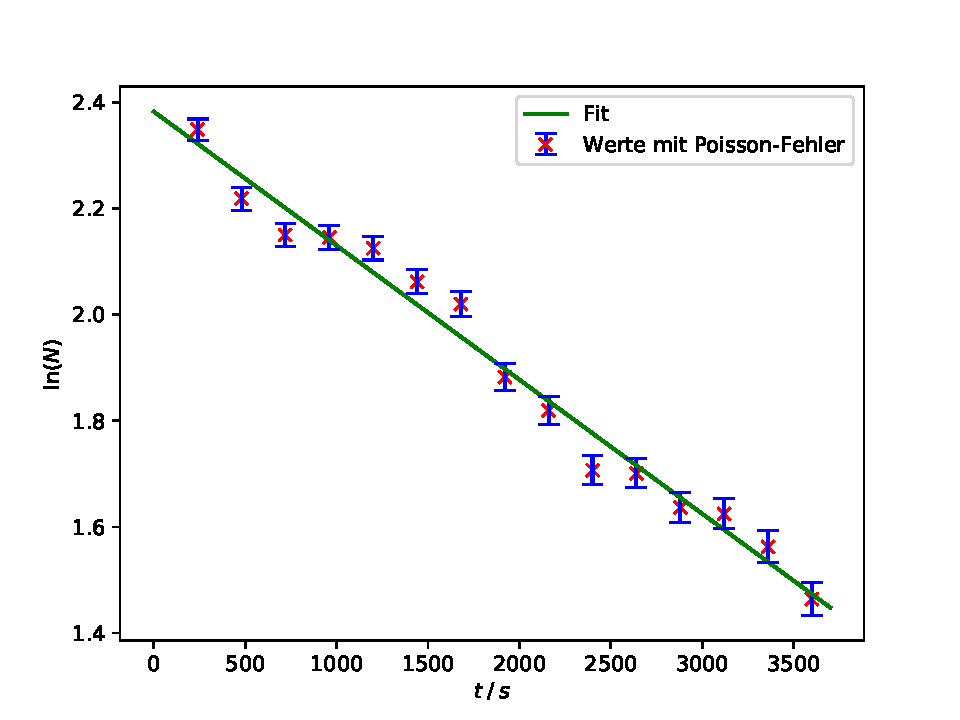
\includegraphics[width=\textwidth]{Plots/ind.pdf}
  \caption{Zerfallskurve von $\ce{^{116}In}$}
  \label{fig:ind}
\end{figure}

Eine lineare Regression $f(x) = -a \cdot x + b$ liefert die Werte
\begin{align*}
  a &= \SI{2,52(10)e-4}{\per \s} \\
  b &= \SI{2,38(2)}{}
\end{align*}

Die Halbwertszeit des Indium-Isotops beträgt somit
\begin{equation*}
  \tau_{\ce{^{116}In}} = \frac{\ln(2)}{a} = \SI{45,76(179)}{\min}.
\end{equation*}

Der Fehler ergibt sich aus der Gauß'schen Fehlerfortpflanzung
\begin{equation}
  \symup{\Delta} \tau_{\ce{^{116}In}} = \sqrt{\left(-\frac{\ln{(2)}}{a^2} \cdot \symup{\Delta}a \right)^2}
\end{equation}

Der Theoriewert \cite{sample2} ist $\tau_{\ce{^{116}In}, \text{theo}} = \SI{54,29}{\min}$. Die Abweichung liegt bei $15,72 \%$.

Außerdem ergibt sich
\begin{equation*}
  N_0 \left(1 - e^{-\symup{\Delta}t a} \right) = \SI{10,83(23)}{\becquerel}.
\end{equation*}

\subsection{Rhodium \label{sec:rhod}}

In Tabelle \ref{tab:rhod} befinden sich die aufgenommenen Messwerte, bei denen der Nulleffekt von $\SI{0,25}{\per \s}$ bereits berücksichtigt wurde.
\begin{longtable}{ c c c S S S }
  \caption{Aufgenommene Messwerte des Rhodium-Zerfalls unter Berücksichtigung des Nulleffekts mit der berechneten Logarithmierung und ihren Abweichungen}
  \label{tab:rhod} \\
  \toprule
  {$t\:/\: \mathrm{s}$} & {$N$} & {$N\:/\: \mathrm{Bq}$} & {$\ln{(N)}$} & {$\ln{(N+\sigma)}-\ln{(N)}$} & {$\ln{(N)}-\ln{(N-\sigma)}$} \\
  \midrule
 \endfirsthead
  \caption{Aufgenommene Messwerte des Rhodium-Zerfalls unter Berücksichtigung des Nulleffekts mit der berechneten Logarithmierung und ihren Abweichungen (Fortsetzung)} \\
 \toprule
 {$t\:/\: \mathrm{s}$} & {$N$} & {$N\:/\: \mathrm{Bq}$} & {$\ln{(N)}$} & {$\ln{(N+\sigma)}-\ln{(N)}$} & {$\ln{(N)}-\ln{(N-\sigma)}$} \\
  \midrule
 \endhead
  \midrule
 \endfoot
  \bottomrule
 \endlastfoot
    18 & 602 & 33,19\pm1,36 & 3,50 & 0,04 & 0,04 \\
    36 & 507 & 27,92\pm1,25 & 3,33 & 0,04 & 0,05 \\
    54 & 371 & 20,36\pm1,06 & 3,01 & 0,05 & 0,05 \\
    72 & 297 & 16,25\pm0,95 & 2,79 & 0,06 & 0,06 \\
    90 & 232 & 12,64\pm0,84 & 2,54 & 0,06 & 0,07 \\
    108 & 201 & 10,92\pm0,78 & 2,39 & 0,07 & 0,07 \\
    126 & 172 & 9,31\pm0,72 & 2,23 & 0,07 & 0,08 \\
    144 & 115 & 6,14\pm0,58 & 1,81 & 0,09 & 0,10 \\
    162 & 122 & 6,53\pm0,60 & 1,88 & 0,09 & 0,10 \\
    180 & 87 & 4,58\pm0,50 & 1,52 & 0,10 & 0,12 \\
    198 & 79 & 4,14\pm0,48 & 1,42 & 0,11 & 0,12 \\
    216 & 57 & 2,92\pm0,40 & 1,07 & 0,13 & 0,15 \\
    234 & 74 & 3,86\pm0,46 & 1,35 & 0,11 & 0,13 \\
    252 & 57 & 2,92\pm0,40 & 1,07 & 0,13 & 0,15 \\
    270 & 55 & 2,81\pm0,39 & 1,03 & 0,13 & 0,15 \\
    288 & 46 & 2,31\pm0,36 & 0,84 & 0,14 & 0,17 \\
    306 & 50 & 2,53\pm0,37 & 0,93 & 0,14 & 0,16 \\
    324 & 40 & 1,97\pm0,33 & 0,68 & 0,16 & 0,18 \\
    342 & 48 & 2,42\pm0,37 & 0,88 & 0,14 & 0,16 \\
    360 & 32 & 1,53\pm0,29 & 0,42 & 0,17 & 0,21 \\
    378 & 40 & 1,97\pm0,33 & 0,68 & 0,16 & 0,18 \\
    396 & 34 & 1,64\pm0,30 & 0,49 & 0,17 & 0,20 \\
    414 & 31 & 1,47\pm0,29 & 0,39 & 0,18 & 0,22 \\
    432 & 16 & 0,64\pm0,19 & -0,45 & 0,26 & 0,35 \\
    450 & 26 & 1,19\pm0,26 & 0,18 & 0,20 & 0,24 \\
    468 & 38 & 1,86\pm0,32 & 0,62 & 0,16 & 0,19 \\
    486 & 25 & 1,14\pm0,25 & 0,13 & 0,20 & 0,25 \\
    504 & 34 & 1,64\pm0,30 & 0,49 & 0,17 & 0,20 \\
    522 & 34 & 1,64\pm0,30 & 0,49 & 0,17 & 0,20 \\
    540 & 25 & 1,14\pm0,25 & 0,13 & 0,20 & 0,25 \\
    558 & 20 & 0,86\pm0,22 & -0,15 & 0,23 & 0,29 \\
    576 & 23 & 1,03\pm0,24 & 0,03 & 0,21 & 0,26 \\
    594 & 17 & 0,69\pm0,20 & -0,36 & 0,25 & 0,33 \\
    612 & 15 & 0,58\pm0,18 & -0,54 & 0,27 & 0,37 \\
    630 & 24 & 1,08\pm0,25 & 0,08 & 0,20 & 0,26 \\
    648 & 14 & 0,53\pm0,17 & -0,64 & 0,28 & 0,39 \\
    666 & 18 & 0,75\pm0,20 & -0,29 & 0,24 & 0,32 \\
    684 & 22 & 0,97\pm0,23 & -0,03 & 0,21 & 0,27 \\
    702 & 19 & 0,81\pm0,21 & -0,22 & 0,23 & 0,30 \\
    720 & 18 & 0,75\pm0,20 & -0,29 & 0,24 & 0,32 \\
    738 & 20 & 0,86\pm0,22 & -0,15 & 0,23 & 0,29 \\
    756 & 17 & 0,69\pm0,20 & -0,36 & 0,25 & 0,33 \\
    774 & 17 & 0,69\pm0,20 & -0,36 & 0,25 & 0,33 \\
\end{longtable}


Zuerst wird die Zerfallskurve des langlebigen Zerfalls $\ce{^{104i}Rh}$ bestimmt.
In Abbildung \ref{fig:r1} sind die Werte für $t \geq \SI{468}{\s}$ aufgetragen.
\begin{figure}[H]
  \centering
  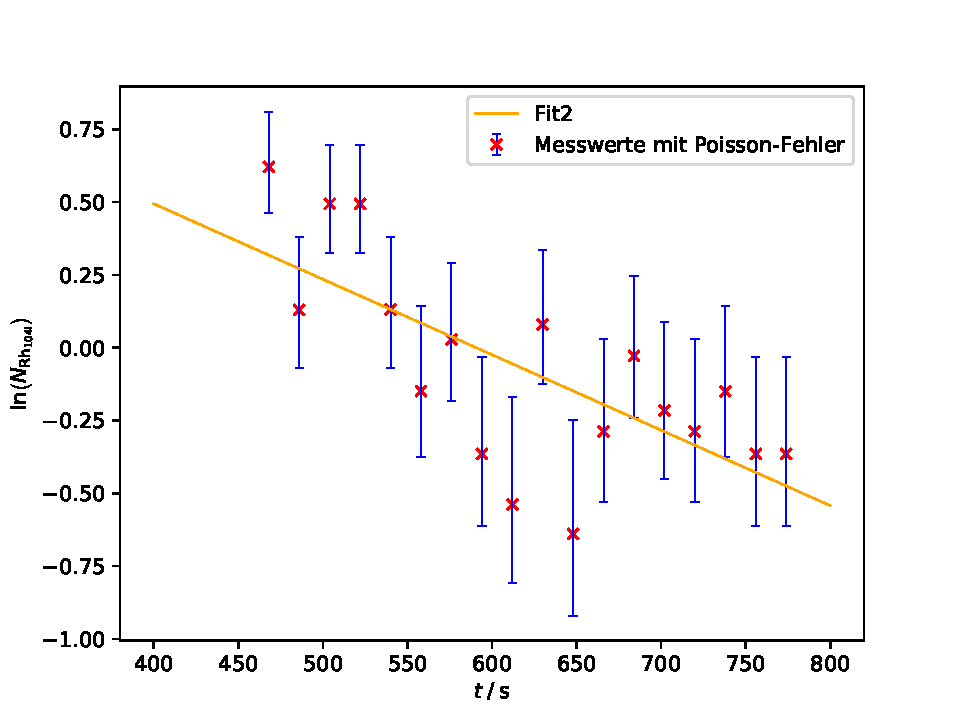
\includegraphics[width=\textwidth]{Plots/rhodi.pdf}
  \caption{Zerfallskurve von $\ce{^{104i}Rh}$}
  \label{fig:r1}
\end{figure}

Aus einer linearen Regression $f(x) = -a \cdot x + b$ mit
\begin{align*}
  a &= \SI{2,6(7)e-3}{\per \s} \\
  b &= \SI{4,6(119)}{}
\end{align*}

mit der Gauß'schen Fehlerfortpflanzung \eqref{eqn:err1}
\begin{equation}
  \symup{\Delta} \tau_{\ce{^{104i}Rh}} = \sqrt{\left(-\frac{\ln{(2)}}{a^2} \cdot \symup{\Delta}a \right)^2}
  \label{eqn:err1}
\end{equation}

ergibt sich die Halbwertszeit
\begin{equation*}
  \tau_{\ce{^{104i}Rh}} = \frac{\ln(2)}{a} = \SI{270(70)}{\s}.
\end{equation*}

Der Theoriewert \cite{sample3} liegt bei $\tau_{\ce{^{104i}Rh}, \text{theo}} = \SI{260}{\s}$, somit beträgt die Abweichung $3,85 \%$.

Beim kurzlebigen Zerfall $t \leq \SI{216}{\s}$ gilt
\begin{equation*}
  \ln{\left(N_{\ce{^{104}Rh}}\right)} = \ln{\left(N_\text{ges} - N_{\ce{^{104i}Rh}}\right)} = -c \cdot x + d.
\end{equation*}

Dies ist in Abbildung \ref{fig:r2} dargestellt.
\begin{figure}[H]
  \centering
  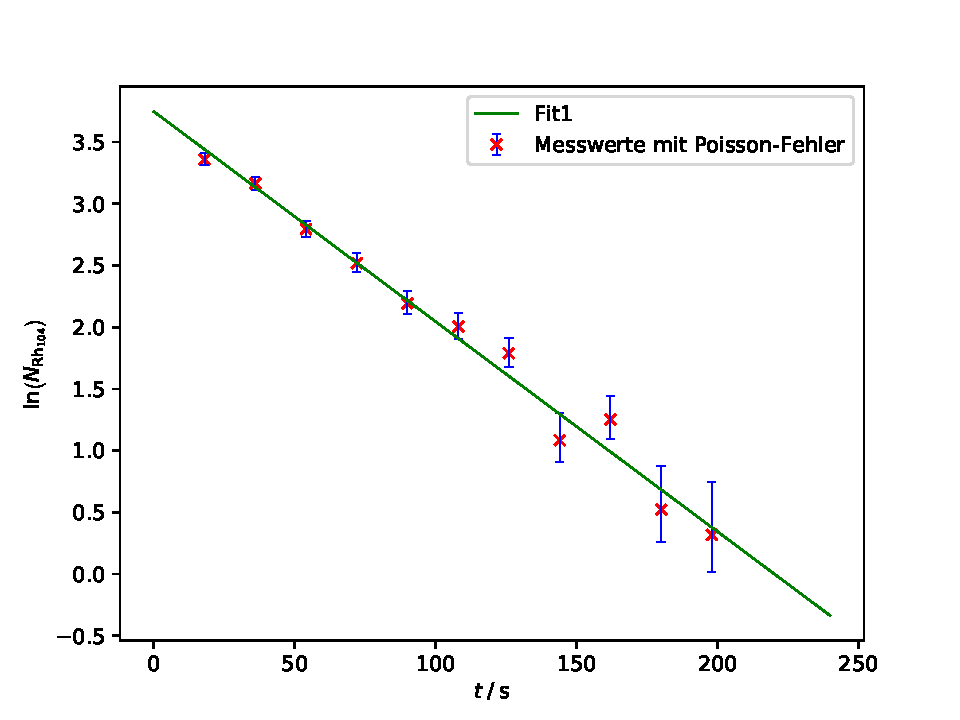
\includegraphics[width=\textwidth]{Plots/rhod.pdf}
  \caption{Zerfallskurve von $\ce{^{104}Rh}$}
  \label{fig:r2}
\end{figure}

Für die Parameter der linearen Regression ergibt sich
\begin{align*}
  c &= \SI{17,0(8)e-3}{\per \s} \\
  d &= \SI{42(4)}{}.
\end{align*}

Mit der Gauß'schen Fehlerfortpflanzung \eqref{eqn:err2}
\begin{equation}
  \symup{\Delta} \tau_{\ce{^{104}Rh}} = \sqrt{\left(-\frac{\ln{(2)}}{c^2} \cdot \symup{\Delta}c \right)^2}
  \label{eqn:err2}
\end{equation}

ergibt sich die Halbwertszeit
\begin{equation*}
  \tau_{\ce{^{104}Rh}} = \frac{\ln(2)}{c} = \SI{40,7(19)}{\s}.
\end{equation*}

Der Theoriewert \cite{sample3} liegt bei $\tau_{\ce{^{104}Rh}, \text{theo}} = \SI{42}{\s}$, somit beträgt die Abweichung $3,10 \%$.

Für die gesamte Zerfallskurve gilt
\begin{equation*}
  N(t) = N_{\ce{^{104}Rh}} + N_{\ce{^{104i}Rh}}.
\end{equation*}

Diese ist in Graph \ref{fig:r3} halblogarithmisch aufgetragen und zusammen mit den bereits in Abbildung \ref{fig:r1} und \ref{fig:r2}
gezeigten Regressionen dargestellt.
\begin{figure}[H]
  \centering
  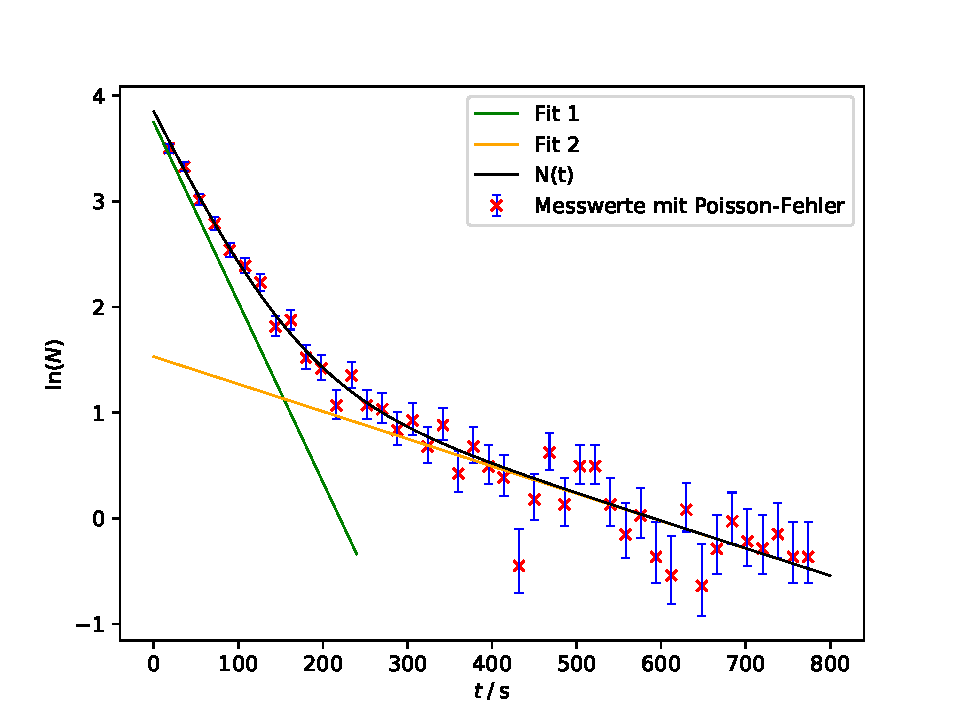
\includegraphics[width=\textwidth]{Plots/rhodges.pdf}
  \caption{Die gesamte Zerfallskurve bei halblogarithmischer Auftragung}
  \label{fig:r3}
\end{figure}

In Abbildung \ref{fig:r4} ist $N(t)$ nochmals aufgetragen, dieses mal aber bei linearer Auftragung.
\begin{figure}[H]
  \centering
  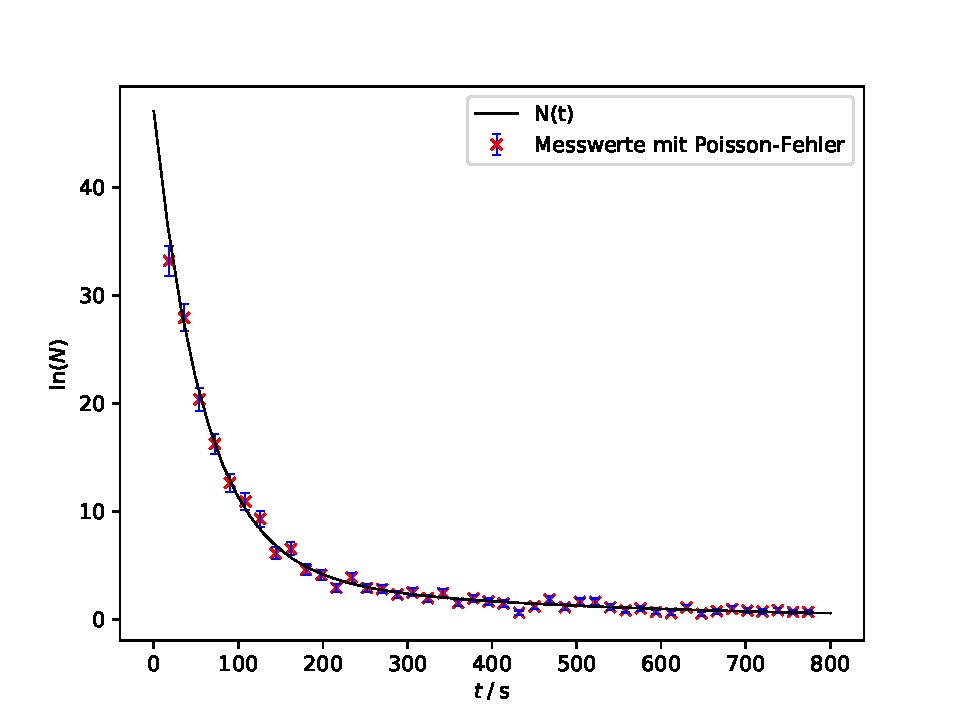
\includegraphics[width=\textwidth]{Plots/rhodgesnolog.pdf}
  \caption{Die gesamte Zerfallskurve}
  \label{fig:r4}
\end{figure}
